% ----------------------------------------------------------
% ESCOPO
% ----------------------------------------------------------
\section{Escopo}

Neste tópico são abordados os casos de uso da aplicação (forma de descrever uma funcionalidade do sistema); diagrama de requisitos (identificação das funcionalidades a serem implementadas); histórias de usuário (descrição das necessidades do usuário); e definição de entregas (quais funcionalidades estarão disponíveis nas principais entregas).
% ----------------------------------------------------------
% REQUISITOS
% ----------------------------------------------------------
\subsection{Requisitos}

Para o desenvolvimento da aplicação \emph{EstagiEI}, são expostos os requisitos funcionais, não-funcionais e regras de negócio que a aplicação terá, tais requisitos foram formados a partir de estudos de como irão funcionar os processos do sistema em construção.

% ----------------------------------------------------------
% REQUISITOS FUNCIONAIS
% ----------------------------------------------------------
\subsubsection{Requisitos Funcionais}

Os requisitos funcionais dizem respeito às principais funcionalidades que o sistema deve empenhar \cite{sommerville}. Durante nossa análise, foram decididos os principais requisitos funcionais da aplicação como descrito no \autoref{req-fun}:

\begin{quadro}[H]
\ABNTEXfontereduzida
\centering
\caption[Requisitos funcionais]{Requisitos funcionais}
    \begin{tabular}{|l|l|}
    \hline
    \multicolumn{1}{|c|}{\textbf{Código}} &
      \multicolumn{1}{c|}{\textbf{Descrição}} \\ \hline
    RF-001 &
      \begin{tabular}[c]{@{}l@{}}Permitir a busca de vagas por filtros\end{tabular} \\ \hline
    RF-002 &
      Recomendar vagas para estudantes \\ \hline
    RF-003 &
      Manter um histórico de vagas tanto para o candidato, quanto para a empresa \\ \hline
    RF-004 & 
      Exibir uma linha do tempo do andamento da vaga \\ \hline
    RF-005 &
      Alertar os estudantes aplicados à vaga sobre cada mudança em seu processo \\ \hline
    RF-006 &
      \begin{tabular}[c]{@{}l@{}}Possibilitar que a empresa entre em contato com os estudantes recomendados \\e/ou aplicados à vaga\end{tabular} \\ \hline
    RF-007 &
      Possibilitar que a empresa realize mudanças no status de andamento da vaga \\ \hline
    RF-008 &
      \begin{tabular}[c]{@{}l@{}}Possibilitar que o estudante realize um \textit{feedback} da empresa pós-entrevista, \\ que será visto por outros estudantes\end{tabular} \\ \hline
    RF-009 &
      \begin{tabular}[c]{@{}l@{}}Não permitir o registro de vagas cujas horas de atividades ultrapassem a carga\\ horária prevista por lei de acordo com a situação escolar de cada estudante\end{tabular} \\ \hline
    RF-010 &
      \begin{tabular}[c]{@{}l@{}}Permitir o cadastro de vagas por parte da empresa, seguindo as regras estabelecidas\end{tabular} \\ \hline
    RF-011 &
      Recomendar estudantes para vagas \\ \hline
	RF-012 &
	  Manter um histórico de vagas para a empresa \\ \hline
	RF-013 & 
	  Possibilitar que a Empresa gerencie suas Vagas \\ \hline
	RF-014 &
	  Possibilitar que a Empresa gerencie seus Representantes \\ \hline
	RF-015 &
	  Possibilitar que a empresa faça um pré-cadastro para ter acesso ao sistema \\ \hline
	RF-016 &
	  Permitir que estudantes se cadastrem no sistema \\ \hline
	RF-017 &
	  \begin{tabular}[c]{@{}l@{}} Possibilitar que estudantes gerenciem o seu perfil, adicionando, alterando e/ou\\ retirando informações. \end{tabular} \\ \hline
	RF-018 &
	  Possibilitar que os estudantes possam se candidatarem à uma vaga. \\ \hline
	RF-019 &
	  Possibilitar que  os estudantes possam retirar suas candidaturas às vagas. \\ \hline
	RF-020 &
	  \begin{tabular}[c]{@{}l@{}} Possibilitar que a empresa visualize facilmente as informações das suas vagas e \\candidaturas aplicadas à elas \end{tabular} \\ \hline
	RF-021 &
	  Possibilitar que o Administrador do sistema possa gerenciar as empresas \\ \hline
	RF-022 &
	  Possibilitar que o Administrador entre em contato com o estudante \\ \hline
	RF-023 &
	  Possibilitar que o Administrador entre em contato com a empresa \\ \hline
    \end{tabular}
    \fonte{Os Autores}
    \label{req-fun}
\end{quadro}

% ----------------------------------------------------------
% REQUISITOS NÃO-FUNCIONAIS
% ----------------------------------------------------------
\subsubsection{Requisitos Não-funcionais}

Ao contrário dos requisitos funcionais, os requisitos não-funcionais não estão ligados às principais funcionalidades de um sistema, mas sim com seus fatores de restrições e especificações. É a partir deles que são observados aspectos como desempenho, usabilidade, segurança e outros aspectos não-funcionais que tangem o sistema \cite{sommerville}.
Tendo isto em mente, no \autoref{req-nao-fun} são elencados os principais requisitos não-funcionais. 
\begin{quadro}[H]
\centering
\ABNTEXfontereduzida
\caption[Requisitos não funcionais]{Requisitos não-funcionais}
    \begin{tabular}{|l|l|}
    \hline
    \multicolumn{1}{|c|}{\textbf{Código}} & \multicolumn{1}{c|}{\textbf{Descrição}}                                 \\ \hline
    RNF-001                               & O sistema deve oferecer boa usabilidade (Ser fácil de aprender a usar)  \\ \hline
    RNF-002                               & O sistema deve estar disponível 24 horas por dia, 7 dias por semana     \\ \hline
    RNF-003                               & O sistema deve possuir possibilidade de escalabilidade                  \\ \hline
    RNF-004                               & Tempo para o carregamento que satisfaça as expectativas do cliente      \\ \hline
    RNF-005                               & O sistema deve possuir uma taxa de ocorrência de falhas menor que 0.3\% \\ \hline
    RNF-006                               & O sistema deve estar de acordo com a \ac{lgpd}                          \\ \hline
    RNF-007 & \begin{tabular}[c]{@{}l@{}}O sistema deve estar de acordo com a lei Nº 11.788, de 25 de setembro de 2008, \\ regulando a carga horária do estágio\end{tabular} \\ \hline
    RNF-008 & \begin{tabular}[c]{@{}l@{}}O sistema deve ser responsivo aos diferentes dispositivos que os usuários \\ podem utilizar para acessá-lo\end{tabular}             \\ \hline
    \end{tabular}
    \fonte{Os Autores}
    \label{req-nao-fun}
\end{quadro}

% ----------------------------------------------------------
% REGRAS DE NEGÓCIO
% ----------------------------------------------------------
\subsubsection{Regras de Negócio}
As regras de negócio, que estão ligadas aos requisitos funcionais previamente descritos, do nosso projeto estão listados no \autoref{regra-negocio}.

\begin{quadro}[H]
\centering
\ABNTEXfontereduzida
\caption[Regras de negócio]{Regras de negócio}
    \begin{tabular}{|l|l|l|}
    \hline
    \multicolumn{1}{|c|}{\textbf{Código}} &
      \multicolumn{1}{c|}{\textbf{Descrição}} &
      \multicolumn{1}{c|}{\textbf{Requisito Relacionado}} \\ \hline
    RN-001 &
      \begin{tabular}[c]{@{}l@{}}As vagas a serem cadastradas devem estar \\ coerentes com o perfil buscado\end{tabular} &
      RF-010 \\ \hline
    RN-002 &
      \begin{tabular}[c]{@{}l@{}}Os históricos das vagas devem ser mantidos \\ por todo o período\end{tabular} &
      RF-003 \\ \hline
    RN-003 &
      \begin{tabular}[c]{@{}l@{}}A empresa é responsável pelo encaminhamento \\ do status da vaga\end{tabular} &
      RF-007 \\ \hline
    RN-004 &
      \begin{tabular}[c]{@{}l@{}}Para o candidato enviar um \textit{feedback}, ele deve \\ ter pelo menos iniciado o processo seletivo\end{tabular} &
      RF-008 \\ \hline
    RN-005 &
      \begin{tabular}[c]{@{}l@{}}O \textit{feedback} pode ser feito de forma anônima, mas o \\ usuário deve estar logado e ter passado pelo processo \\ seletivo\end{tabular} &
      RF-008 \\ \hline
    RN-006 &
      \begin{tabular}[c]{@{}l@{}}A recomendação de vagas deve ocorrer para estudantes\\ devidamente cadastrados que possuam ao menos uma\\ competência em seu perfil.\end{tabular} &
      RF-002 \\ \hline
    \end{tabular}
    \fonte{Os Autores}
    \label{regra-negocio}
\end{quadro}

% ----------------------------------------------------------
% HISTÓRIAS DE USUÁRIO
% ----------------------------------------------------------
\subsection{Histórias de usuário}

A seguir apresentamos as histórias de usuário da aplicação, divididas entre os \textit{Epics}. Primeiro as histórias relacionadas ao \textit{Epic} da Empresa em \autoref{user-story-company}, posteriormente o do Estudante em \autoref{user-story-student} e por fim do Administrador em \autoref{user-story-admin}.

\begin{quadro}[H]
	\centering
	\ABNTEXfontereduzida
	\caption{Histórias de usuário - Empresa}
	\label{user-story-company}
	\begin{tabular}{|l|l|p{9cm}|}
	\hline
		\thead{Código} & \thead{Nome} & \thead[l]{Descrição}\\
	\hline
	H001 & Cadastrar Vagas &
		Como empresa, eu quero poder gerenciar (cadastrar, editar, visualizar detalhes, listar) vagas dentro do sistema para poder deixá-las visíveis e acessíveis para possíveis candidatos.  \\
	\hline
	H002 & Detalhes da Vaga & (Idem H001) \\
	\hline
	H003 & Abrir Candidaturas & Como empresa, eu quero ter a possibilidade de abrir as candidaturas para uma vaga para que estudantes possam se candidatar. \\
	\hline
	H004 & Fechar Candidaturas & Como empresa, eu quero ter a possibilidade de fechar as candidaturas para uma vaga para que estudantes não possam mais se candidatar. \\
	\hline
	H005 & Editar Vagas & (Idem H001) \\
	\hline
	H006 & Excluir Vagas & Como empresa, eu quero poder excluir uma vaga para retirá-la de visualização completamente. \\
	\hline
	H007 & Listar Vagas & (Idem H001)\\
	\hline
	H008 & Receber Recomendações & Como empresa, eu quero receber recomendações de estudantes para as vagas para que a busca por candidatos seja facilitada. \\
	\hline
	H009 & Histórico de Candidaturas & Como empresa, eu quero um histórico dos estudantes que se candidataram às vagas para que eu possa contactá-los se necessário para aquela vaga ou outras ainda em aberto.  \\
	\hline
	H010 & Dashboard de Visualização & Como empresa, eu quero uma forma rápida e fácil de visualizar as informações pertinentes às minhas vagas para gerenciá-las. \\
	\hline
	H011 & Cadastrar Representantes & Como empresa, eu quero gerenciar (cadastrar, editar, ver detalhes, listar) representantes para que eu tenha melhor controle e conhecimento daqueles que podem gerenciar minhas vagas por mim. \\
	\hline
	H012 & Detalhes do Representante & (Idem H011) \\
	\hline
	H013 & Editar Representantes & (Idem H011) \\
	\hline
	H014 & Excluir Representante & Como empresa, eu quero excluir um representante para que este não possa mais acessar o sistema em meu nome nem gerenciar minhas vagas. \\
	\hline
	H015 & Listar Representantes & (Idem H011) \\
	\hline
	H016 & Login Representantes & Como empresa, eu quero autorizar que um representante entre no sistema em meu nome para que este representante gerencie minhas vagas. \\
	\hline
	H017 & Solicitar Cadastro no site & Como empresa, eu quero poder solicitar meu cadastro no site para ter acesso ao sistema.\\
	\hline
	H018 & Contato com Estudante & Como empresa, eu quero me comunicar de forma fácil com os estudantes candidatos para que o processo seja mais ágil. \\
	\hline
	H019 & Solicitar exclusão da Conta & Como empresa, eu quero poder solicitar a exclusão da minha conta e todos os meus dados para que minha propriedade sobre eles seja respeitada, de acordo com a LGPD. \\
	\hline
	
	\end{tabular}
	\fonte{Os autores}
\end{quadro}

\begin{quadro}[H]
	\centering
	\ABNTEXfontereduzida
	\caption{Histórias de usuário - Estudante}
	\label{user-story-student}
	\begin{tabular}{|l|p{4cm}|p{9cm}|}
		\hline 
		\thead{Código} & \thead[l]{Nome} & \thead[l]{Descrição} \\
		\hline
		H020 & Buscar Vagas & Como estudante, eu quero buscar vagas podendo usar de filtros para facilitar minha pesquisa e escolha de vaga. \\
		\hline
		H021 & Receber Recomendações & Como estudante, eu quero receber recomendações de vaga para que a minha pesquisa seja facilitada.\\
		\hline
		H022 & Candidatar-se à Vaga & Como estudante, eu quero poder me candidatar à uma vaga para ter a chance de ser selecionado para um estágio. \\
		\hline
		H023 & Retirar Candidatura & Como estudante, eu quero poder retirar minha candidatura para uma vaga para que eu não possa ser selecionado para ela. \\
		\hline
		H024 & Listar Candidaturas & Como estudante, eu quero um histórico de todas as minhas vagas já aplicadas para poder gerenciá-las melhor. \\
		\hline
		H025 & Acompanhar Etapas & Como estudante, eu quero uma linha do tempo com os principais passos do processo para que eu possa acompanhá-lo de forma fácil e rápida.\\
		\hline
		H026 & Notificação de Mudança na Vaga & Como estudante, eu quero ser alertado sobre as mudanças no status da vaga para que possa saber de forma rápida sua situação. \\
		\hline
		H027 & Denunciar Vagas & Como estudante, eu quero poder denunciar vagas que possuam algum tipo de irregulariedade para que elas sejam retiradas do sistema. \\
		\hline
		H028 & Buscar Empresas & Como estudante, eu quero poder buscar as empresas cadastradas no site para facilitar minha busca pelas vagas pertencentes àquela empresa. \\
		\hline
		H029 & Detalhes de uma Empresa & Como estudante, eu quero poder ver os detalhes de uma empresa para poder decidir se suas vagas podem vir a me interessar ou não. \\
		\hline
		H030 &  Vagas de uma empresa & Como estudante, eu quero poder ver as vagas de uma empresa específica para facilitar a minha busca. \\
		\hline
		H031 & Dar Feedback & Como estudante, eu quero poder dar um feedback sobre o processo seletivo/empresa da qual participei da seleção/estágio para que outros utilizadores do site tenham mais informações sobre aquela empresa. \\
		\hline
		H032 & Detalhes do Perfil & Como estudante, eu quero ver os detalhes do meu perfil para verifiar as informações contidas ali. \\
		\hline
		H033 & Editar Perfil & Como estudante, eu quero editar o meu perfil para melhorar/atualizar/corrigir as informações apresentadas. \\
		\hline
		H034 & Adicionar Competências & Como estudante, eu quero poder gerenciar (adicionar, retirar, ver todas) as competências do meu perfil para mantê-lo atualizado e/ou direcionar as recomendações de vagas. \\
		\hline
		H035 & Retirar Competências & (Idem H034) \\
		\hline
		H036 & Listar Competências & (Idem H034) \\
		\hline
		H037 & Solicitar exclusão da Conta & Como estudante, eu quero poder solicitar a exclusão da minha conta e todos os meus dados para que minha propriedade sobre eles seja respeitada, de acordo com a LGPD. \\
		\hline
		H038 & Cadastro no site & Como estudante, eu quero poder me cadastrar no site para poder ter acesso ao sistema. \\
		\hline
		H039 & Login & Como estudante, eu quero poder fazer login no site para ter acesso às funcionalidades do sistema. \\
		\hline
	\end{tabular}
\fonte{Os autores}
\end{quadro}

\begin{quadro}[H]
	\centering
	\ABNTEXfontereduzida
	\caption{Histórias de usuário - Administrador}
	\label{user-story-admin}
	\begin{tabular}{|l|p{4 cm}|p{9 cm}|}
		\hline 
		\thead{Código} & \thead[l]{Nome} & \thead[l]{Descrição} \\
		\hline
		H040 & Cadastrar Empresa & Como Admin, eu quero poder gerenciar (cadastrar, editar, ver detalhes) as empresas do site para ter um melhor controle de quem está oferecendo vagas de estágio. \\
		\hline
		H041 & Editar Empresa & (Idem H040) \\
		\hline
		H042 & Página da Empresa & (Idem H040) \\
		\hline
		H043 & Excluir Empresa & Como Admin, eu quero poder excluir uma conta de empresa e todos os seus dados para cumprir com a LGPD quando houver uma solicitação condizente. \\
		\hline
		H044 & Receber Denúncias & Como Admin, eu quero receber as denúncias feitas por estudantes para facilitar a busca por vagas inadequadas no sistema. \\
		\hline
		H045 & Excluir Vagas Inadequadas & Como Admin, eu quero poder excluir vagas inadequadas do sistema para deixá-lo o mais condizente com a lei e com as necessidades dos estudantes. \\
		\hline
		H046 & Contato com Estudante & Como Admin, eu quero ter contato fácil com os estudantes para transmitir informações pertinentes sobre o sistema e as vagas. \\
		\hline
		H047 & Contato com a Empresa & Como Admin, eu quero ter contato fácil com as empresas para transmitir informações pertinentes sobre o sistema e as vagas. \\
		\hline
		H048 & Receber solicitações de exclusão de Contas & Como Admin, eu quero receber solicitações de exclusão de contas dos usuários para poder cumprir com as determinações da LGPD.. \\
		\hline
		H049 & Excluir Perfil/Conta do Estudante & Como Admin, eu quero poder excluir uma conta de estudante e todos os seus dados para cumprir com a LGPD quando houver uma solicitação condizente. \\
		\hline
	\end{tabular}
	\fonte{Os autores}
\end{quadro}

Cada história de usuário está relacionada com um caso de uso, os quais serão explicados melhor a seguir, e com algum requisito e/ou regra de negócio. As relações são indicadas de modo mais detalhado no <AUTO-REFERENCIAR APÊNDICE>.

\subsection{Casos de uso}

A \autoref{casotodos} mostra os casos de uso que são pertinentes a aplicação, demonstrando os principais atores e suas funcionalidades dentro do sistema.


\begin{figure}[H]
	\centering
	\caption{\label{casotodos}Caso de Uso - EstagiEI}
	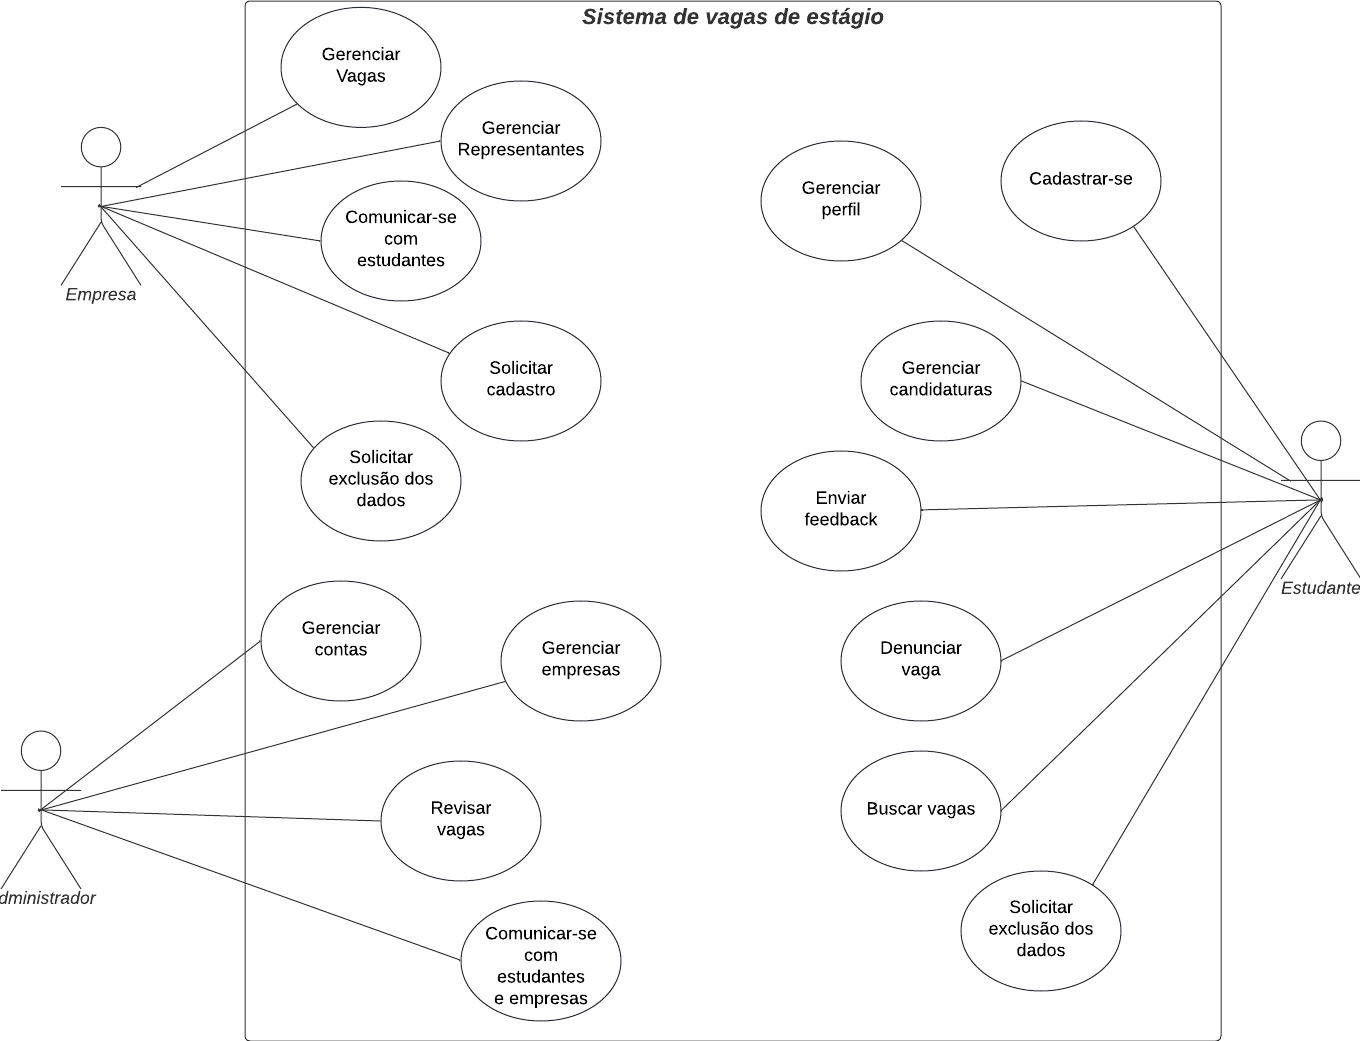
\includegraphics[width=0.8\textwidth]{../imagens/caso-de-uso.png}
	\fonte{Os Autores}
\end{figure}

O \autoref{user-cases} mostra os mesmos casos de uso outra forma, associando cada caso com um código que será usado em <AUTO-REFERENCIAR APÊNDICE>, relacionando com as histórias de usuário, requisitos e regras de negócio.

\begin{quadro}[H]
	\centering
	\ABNTEXfontereduzida
	\caption{Casos de uso}
	\label{user-cases}
	\begin{tabular}{|l|p{4 cm}|p{9 cm}|}
		\hline 
		\thead{Código} & \thead[l]{Ator} & \thead[l]{Descrição} \\
		\hline
		UC001 & Empresa & Gerenciar Representantes\\
		\hline
		UC002 & Empresa & Cadastrar a Vaga \\
		\hline
		UC003 & Empresa & Gerenciar a Vaga \\
		\hline
		UC004 & Empresa & Mudar Status da Vaga \\
		\hline
		UC005 & Estudante & Buscar Vagas \\
		\hline
		UC006 & Estudante & Gerenciar Candidaturas \\
		\hline
		UC007 & Estudante & Denunciar Vaga \\
		\hline
		UC008 & Estudante & Enviar Feedbak sobre a empresa \\
		\hline
		UC009 & Admin & Moderar as Vagas oferecidas no sistema \\
		\hline
		UC010 & Admin & Gerenciar Contas \\
		\hline
		UC011 & Admin & Gerenciar Empresas \\
		\hline
		UC012 & Empresa & Solicitar cadastro no sistema \\
		\hline
		UC013 & Estudante & Cadastrar-se no sistema \\
		\hline
		UC014 & Empresa/Estudante & Solicitar exclusão dos dados/conta do sistema \\
		\hline
		UC015 & Estudante & Gerenciar Perfil \\
		\hline
		UC016 & Admin & Comunicar-se com Empresas e/ou Estudantes \\
		\hline
		UC017 & Empresa & Comunicar-se com os Estudantes \\
		\hline
	\end{tabular}
	\fonte{Os autores}
\end{quadro}

\subsection{Fases de entrega}

Nessa seção são expostas quais funcionalidades do sistema foram e serão desenvolvidas, tendo em vista as principais fases de entrega da disciplina, sendo elas a \ac{poc}, o \ac{mvp} e a Entrega Final.

\subsubsection{Prova de Conceito (POC)} \label{entrega-poc}

Na fase de \ac{poc}, foram entregues as funcionalidades mais básicas do nosso software. Dentre elas, o cadastro de estudantes via \ac{sso} da \textit{Google}, onde é explicado o processo no site possibilitando a criação de uma conta com informações básicas, necessárias apenas para o funcionamento padrão do sistema, e o cadastro de empresas, que será feito no próprio sistema \emph{EstagiEI}, onde a empresa preenche as informações e passa por uma aprovação da equipe. Além disso, o software permite o \textit{login} desses usuários já cadastrados, onde poderão consultar suas informações básicas.

Ao se cadastrar no sistema, a empresa também poderá registrar uma pessoa do \ac{rh}, que será responsável por gerenciar as vagas daquela organização, e essa pessoa poderá criar novas vagas com informações básicas, apenas para serem visíveis na tela de consulta de vagas. Na parte do estudante, será possível para ele(a), consultar as vagas que existem no sistema através de filtros básicos e internacionalização de linguagem.

\subsubsection{Produto Mínimo Viável (MVP)}

Na entrega do \ac{mvp}, foi incrementado o que já foi desenvolvido durante a \ac{poc} com funcionalidades importantes ao nosso sistema, como a recomendação de vagas ao estudante e edição de perfil. Além disso, foram feitos os testes unitários e validações de segurança, \ac{html}, testes de interface, etc. A fim de garantir que a aplicação esteja em conforme com os requisitos solicitados.

\subsubsection{Entrega Final}

Na entrega final, serão acrescidos no nosso projeto o que já foi feito antes com o restante das funcionalidades, tais como a possibilidade do estudante denunciar uma vaga por não ser coerente com a proposta da nossa aplicação, que é ser um sistema que possua vagas de estágio coerentes com a realidade de um estagiário; recomendação de candidatos para empresas; opção de contato com o candidato via \textit{Whatsapp}; \textit{dashboard} de vagas para a empresa; histórico de vagas para os estudantes; mudança de \textit{status} das vagas por parte da empresa; \textit{feedback} de empresas após o processo seletivo; e acessibilidade com o \gls{vlibras}.